\documentclass[12pt,a4paper]{article}

%\usepackage[left=1.5cm,right=1.5cm,top=1cm,bottom=2cm]{geometry}
\usepackage[in, plain]{fullpage}
\usepackage{array}
%\usepackage{../../pas-math}
\usepackage{../../moncours}



%-------------------------------------------------------------------------------
%          -Packages nécessaires pour écrire en Français et en UTF8-
%-------------------------------------------------------------------------------
\usepackage[utf8]{inputenc}
\usepackage[frenchb]{babel}
%\usepackage{numprint}
\usepackage[T1]{fontenc}
%\usepackage{lmodern}
\usepackage{textcomp}
\usepackage[french, boxed]{algorithm2e}
\usepackage{hyperref}


%-------------------------------------------------------------------------------

%-------------------------------------------------------------------------------
%                          -Outils de mise en forme-
%-------------------------------------------------------------------------------
\usepackage{hyperref}
\hypersetup{pdfstartview=XYZ}
%\usepackage{enumerate}
\usepackage{graphicx}
\usepackage{multicol}
\usepackage{tabularx}
\usepackage{multirow}
\usepackage{color}
\usepackage{eurosym}


\usepackage{anysize} %%pour pouvoir mettre les marges qu'on veut
%\marginsize{2.5cm}{2.5cm}{2.5cm}{2.5cm}

\usepackage{indentfirst} %%pour que les premier paragraphes soient aussi indentés
\usepackage{verbatim}
\usepackage{enumitem}
\usepackage{booktabs}
\usepackage[usenames,dvipsnames,svgnames,table]{xcolor}

\usepackage{variations}

%-------------------------------------------------------------------------------


%-------------------------------------------------------------------------------
%                  -Nécessaires pour écrire des mathématiques-
%-------------------------------------------------------------------------------
\usepackage{amsfonts}
\usepackage{amssymb}
\usepackage{amsmath}
\usepackage{amsthm}
\usepackage{tikz}
\usepackage{xlop}
\usepackage[output-decimal-marker={,}]{siunitx}
%-------------------------------------------------------------------------------

%-------------------------------------------------------------------------------
%                  -Nécessaires pour écrire des formules chimiquess-
%-------------------------------------------------------------------------------

\usepackage[version=4]{mhchem}

%-------------------------------------------------------------------------------
% Pour pouvoir exploiter les fichiers directement dans beamer
\newcommand{\pause}{\ }
%-------------------------------------------------------------------------------
%                    - Mise en forme avancée
%-------------------------------------------------------------------------------

\usepackage{ifthen}
\usepackage{ifmtarg}


\newcommand{\ifTrue}[2]{\ifthenelse{\equal{#1}{true}}{#2}{$\qquad \qquad$}}

%\newcommand{\kword}[1]{\textcolor{red}{\underline{#1}}}
%-------------------------------------------------------------------------------

%-------------------------------------------------------------------------------
%                     -Mise en forme d'exercices-
%-------------------------------------------------------------------------------
%\newtheoremstyle{exostyle}
%{\topsep}% espace avant
%{\topsep}% espace apres
%{}% Police utilisee par le style de thm
%{}% Indentation (vide = aucune, \parindent = indentation paragraphe)
%{\bfseries}% Police du titre de thm
%{.}% Signe de ponctuation apres le titre du thm
%{ }% Espace apres le titre du thm (\newline = linebreak)
%{\thmname{#1}\thmnumber{ #2}\thmnote{. \normalfont{\textit{#3}}}}% composants du titre du thm : \thmname = nom du thm, \thmnumber = numéro du thm, \thmnote = sous-titre du thm

%\theoremstyle{exostyle}
%\newtheorem{exercice}{Exercice}
%
%\newenvironment{questions}{
%\begin{enumerate}[\hspace{12pt}\bfseries\itshape a.]}{\end{enumerate}
%} %mettre un 1 à la place du a si on veut des numéros au lieu de lettres pour les questions 
%-------------------------------------------------------------------------------

%-------------------------------------------------------------------------------
%                    - Mise en forme de tableaux -
%-------------------------------------------------------------------------------

\renewcommand{\arraystretch}{1.7}

\setlength{\tabcolsep}{1.2cm}

%-------------------------------------------------------------------------------



%-------------------------------------------------------------------------------
%                    - Racourcis d'écriture -
%-------------------------------------------------------------------------------
%Droites
\newcommand{\dte}[1]{$(#1)$}
\newcommand{\fig}[1]{figure $#1$}
\newcommand{\sym}{symétrique}
\newcommand{\syms}{symétriques}
\newcommand{\asym}{axe de symétrie}
\newcommand{\asyms}{axes de symétrie}
\newcommand{\seg}[1]{$[#1]$}
\newcommand{\monAngle}[1]{$\widehat{#1}$}
\newcommand{\bissec}{bissectrice}
\newcommand{\mediat}{médiatrice}
\newcommand{\ddte}[1]{$[#1)$}


% Angles orientés (couples de vecteurs)
\newcommand{\aopp}[2]{(\vec{#1}, \vec{#2})} %Les deuc vecteurs sont positifs
\newcommand{\aopn}[2]{(\vec{#1}, -\vec{#2})} %Le second vecteur est négatif
\newcommand{\aonp}[2]{(-\vec{#1}, \vec{#2})} %Le premier vecteur est négatif
\newcommand{\aonn}[2]{(-\vec{#1}, -\vec{#2})} %Les deux vecteurs sont négatifs

%Ensembles mathématiques
\newcommand{\naturels}{\mathbb{N}} %Nombres naturels
\newcommand{\relatifs}{\mathbb{Z}} %Nombres relatifs
\newcommand{\rationnels}{\mathbb{Q}} %Nombres rationnels
\newcommand{\reels}{\mathbb{R}} %Nombres réels
\newcommand{\complexes}{\mathbb{C}} %Nombres complexes


%Intégration des parenthèses aux cosinus
\newcommand{\cosP}[1]{\cos\left(#1\right)}
\newcommand{\sinP}[1]{\sin\left(#1\right)}


%Probas stats
\newcommand{\stat}{statistique}
\newcommand{\stats}{statistiques}


\newcommand{\homo}{homothétie}
\newcommand{\homos}{homothéties}


\newcommand{\mycoord}[3]{(\textcolor{red}{\num{#1}} ; \textcolor{Green}{\num{#2}} ; \textcolor{blue}{\num{#3}})}
%-------------------------------------------------------------------------------

%-------------------------------------------------------------------------------
%                    - Mise en page -
%-------------------------------------------------------------------------------

\newcommand{\twoCol}[1]{\begin{multicols}{2}#1\end{multicols}}


\setenumerate[1]{font=\bfseries,label=\textit{\alph*})}
\setenumerate[2]{font=\bfseries,label=\arabic*)}


%-------------------------------------------------------------------------------
%                    - Elements cours -
%-------------------------------------------------------------------------------

%Correction d'exercice
\newcommand{\exoSec}[2]{\subsection*{Exercice #1 page #2}}
%-------------------------------------------------------------------------------
%                    - raccourcis d'écriture -
%-------------------------------------------------------------------------------

%Mise en évidence de termes clés
\newcommand{\mykw}[1]{\textcolor{red}{\underline{\textbf{#1}}}}

%Exercices
\newcommand{\exo}[2]{exercice #1 page #2}
\newcommand{\Exo}[2]{Exercice #1 page #2}

\renewcommand{\pause}{\ }

%Intervalles
\newcommand{\interOO}[2]{$]$#1 , #2$[$}
\newcommand{\interOF}[2]{$]$#1 , #2$]$}
\newcommand{\interFO}[2]{$[$#1 , #2$[$}
\newcommand{\interFF}[2]{$[$#1 , #2$]$}





\date{}
\title{}

\graphicspath{{./img/}}


\begin{document}
	
	
\chap[num=1, color=blue]{\small Quelles sont les deux sortes de sources de lumière ?}{Olivier FINOT, \today }	

\section{Sources de lumière}

\begin{myact}{}
	Activité 19 page 59 cahier d'activités : Différentes formes d'énergie et leurs sources.
	 
	Activité 3 page 136 le livret scolaire : Énergies renouvelables. 
\end{myact}

\begin{mybilan}
	\begin{itemize}
		\item Un \kw{solide} a une \kw{forme propre} qui ne change pas, on peut le saisir.
		\item Un \kw{liquide} prend la \kw{forme du récipient} qui le contient.
		\item La surface d'un liquide en contact avec l'air est sa \kw{surface libre}.
		\item Au repos, cette surface libre est \kw{plane et horizontale}.
	\end{itemize}	   
\end{mybilan}




\begin{myexos}
	\begin{itemize}
		\item \exo{1}{70}
		\item \exo{13}{72}
		\item \exo{17}{73}
	\end{itemize}
\end{myexos}

\section{Voir un objet}

\begin{myact}{2 page 153}
	\begin{enumerate}
		\item Sur la fiole jaugée, le volume est exprimé en millilitres ($mL$). \pause
		\item La fiole jaugée contient \num{1000} $mL$ de liquide, soit 1 litre ($L$). \pause
		\item Le volume du récipient cubique est de 1 décimètre cube ($dm^3$). \pause
		\item On nous indique que le contenu de la fiole jaugée a été transféré sans perdre de liquide, donc le volume n'a pas changé.\pause
		\item Le récipient cubique contient 1 $dm^3$ de liquide, soit \num{1000} centimètres cubes ($cm^3$).\pause
		\item On a 1 $L =$ 1 $dm^3$ et 1 $mL = $ 1 $cm^3$.
	\end{enumerate}
\end{myact}

\begin{mybilan}
	Pour décrire la vitesse d'un objet en mouvement, on utilise trois caractéristiques :
	\begin{itemize}
		\item la \kw{direction} (horizontale, verticale ou oblique), tangente à la trajectoire;
		
		\item le \kw{sens}, celui du mouvement (vers la gauche, vars la droite, vers le haut etc.);
		
		\item la \kw{valeur} exprimée m/s (ou km/h ou autre).
		
		Si le mouvement est uniforme, la relation \kw{$ v = \dfrac{d}{\Delta t} $}, permet de relier la vitesse de l'objet, la distance parcourue et la durée du parcours avec :
		\begin{itemize}
			\item d : distance parcourue en mètre (m)
			\item $\Delta t$ :durée du trajet en seconde (s)
			\item v : vitesse en mètre par seconde (m/s).
		\end{itemize}
	\end{itemize}



\end{mybilan}



\begin{myexos}
	\begin{multicols}{2}
	
		\begin{itemize}
			\item \exo{2}{70}
			\item \exo{6}{71}
			\item \exo{7}{71}
			\item \exo{10}{72}
			\item \exo{11}{72}

		\end{itemize}
	
	\end{multicols}
\end{myexos}


\section{Voir la lumière}

\begin{myact}{3 page 64}
	\begin{enumerate}\pause
		\item Dans une salle obscure, on ne voit pas la lumière entre le projecteur et le cône.\pause
		\item On observe une zone éclairée sur le cône.\pause
		\item Lorsque l'on saupoudre de la craie entre le projecteur et le cône on observe des grains de craie éclairés.\pause
		\item Si les grains ne sont pas dans la lumière, ils n'en reçoivent pas et ne sont donc pas visibles.\pause
		\item Dans cette expérience, les grains de craie sont des objets diffusants.\pause
		\item La lumière n'est visible que si on place des objets diffusants sur son trajet.
	\end{enumerate}
\end{myact}

\begin{mybilan}
	
	\twoCol{
	\begin{center}
		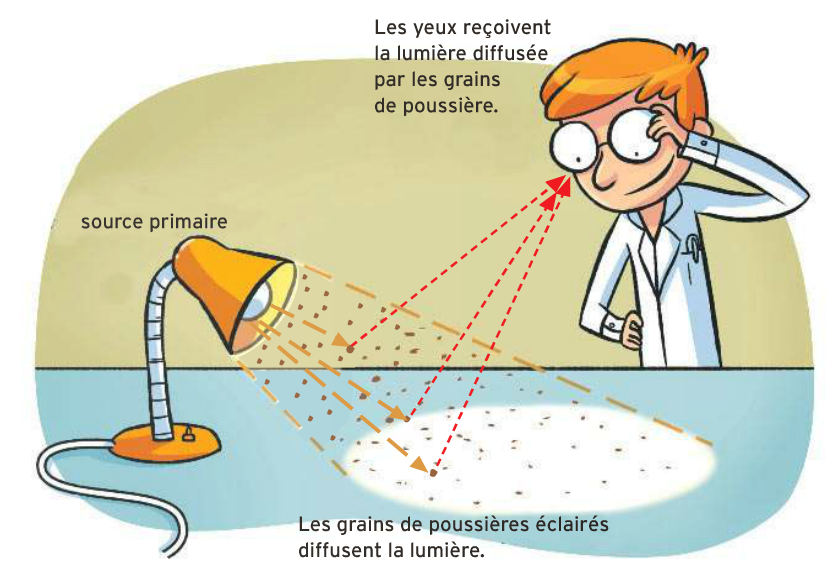
\includegraphics[scale=0.7]{bilan3}
	\end{center}

	\begin{itemize}
		\item Une tension est \kw{périodique} lorsque ses \kw{variations se répètent} identiques à elles mêmes au cours du temps. 
		\item La \kw{durée} d'un motif est la \kw{période}. On la note $T$, son unité est la seconde $s$.
	\end{itemize}
	}

\end{mybilan}

\begin{myexos}
	\begin{itemize}
		\item \exo{3}{70}
		\item \exo{8}{71}
	\end{itemize}
\end{myexos}


\section{Les dangers du rayon laser}



\begin{myact}{4 page 155}
	\begin{enumerate}
		\item L'unité de la température mesurée par la sonde du thermomètre électronique est le degré Celsius (°$C$). \pause
		\item La température du liquide contenu dans le bécher est de \num{17.4} °$C$.\pause
		\item L'intervalle entre deux graduations du thermomètre est alcool correspond à 1 °$C$.\pause
		\item Il faut laisser à la sonde le temps de mesurer précisément la température du liquide, c'est pourquoi on attend que l'affichage se stabilise.\pause
		\item Le réservoir du thermomètre à alcool doit être complètement immergé dans le liquide car c'est lui qui sert à <<mesurer>> la température.\pause
		\item La température mesurée par le thermomètre à alcool est de $17$ °$C$.		
	\end{enumerate}
\end{myact}


\begin{mybilan}
	\begin{itemize}
		\item La masse d'un corps est \kw{proportionnelle} à son volume; \pause
		\item Le coefficient de proportionnalité est la \kw{masse volumique} (notée $\rho$);\pause
		\item \kw{Un litre d'eau} a une masse de \kw{1 kilogramme};\pause
		\item Une substance est \kw{plus dense} qu'une autre si, pour un même volume, sa masse est supérieure.		
	\end{itemize}
\end{mybilan}

\begin{myexos}
	\twoCol{\begin{itemize}
		\item \exo{4}{70}
		\item \exo{9}{71}
		\item \exo{14}{72}
	\end{itemize}}
\end{myexos}
\appendix

\newpage

\section*{Correction des exercices}

\subsection*{\Exo{1}{70}}

\begin{enumerate}[label=\alph*)]
	\item Une lampe allumée est \textbf{une source primaire}.
	\item Les planètes sont des \textbf{objets diffusants}.
	\item Un objet qui renvoie la lumière qu'il reçoit dans toutes les directions est \textbf{un objet diffusant}.
	\item Un objet qui produit la lumière qu'il émet est \textbf{une source primaire}.
\end{enumerate}

\subsection*{\Exo{2}{70}}
	La {source de lumière} (le Soleil) éclaire le livre qui est un \textbf{objet diffusant} et qui renvoie la lumière dans les \textbf{yeux} de la fille.

\subsection*{\Exo{3}{70}}
	La lumière émise par la lampe ne doit pas être visible là où il n'y a pas de poussière.
	
\subsection*{\Exo{4}{70}}

\begin{enumerate}[label=\alph*)]
	\item Un laser est est un faisceau de lumière de \textbf{grande} énergie.
	\item Lorsque le faisceau laser touche un obstacle, on observe un \textbf{minuscule} point d'impact.
	\item Le faisceau laser est  \textbf{dangereux} pour les yeux d'une personne.
	\item On \textbf{ne doit jamais} diriger la lumière d'un pointeur laser vers les yeux d'une personne. 
\end{enumerate}

\subsection*{\Exo{6}{71}}

	Tom doit diriger sa lampe vers l'écran blanc pour que la lumière soit diffusée et renvoyée vers \'Elodie. Ainsi elle sera éclairée.
	
\subsection*{\Exo{7}{71}}
	\begin{enumerate}[label=\alph*)]
		\item La deuxième image (en haut à droite).
		\item Un objet est visible si il est éclairé et renvoie la lumière qu'il reçoit vers les yeux de l'observateur.
	\end{enumerate}

\subsection*{\Exo{8}{71}}
	\begin{enumerate}[label=\alph*)]
		\item On ne voit pas la lumière du projecteur entre celui-ci et le bécher.
		\item Quand on fait bouillir de l'eau il se forme de la vapeur au dessus.
		\item On peut voir le trajet de la lumière car elle est diffusée par les gouttelettes d'eau qui forment la vapeur.
	\end{enumerate}

\subsection*{\Exo{9}{72}}
	\begin{enumerate}[label=\alph*)]
		\item Le panneau indique l'utilisation d'un laser qui peuvent être dangereux.
		\item Les lunettes mises à disposition sont utilisées pour protéger les yeux des observateurs.
	\end{enumerate}

\subsection*{\Exo{10}{72}}
	\begin{enumerate}
		\item La lampe éclaire Tom qui renvoie la lumière vers les yeux d'\'Eric qui peut donc le voir.
		\item Il y a un obstacle opaque, le foulard, entre les yeux de Tom et \'Eric, donc Tom ne peut pas le voir.
		\item Si la lampe est éteinte, il n'y plus de source de lumière principale donc aucun d'eux ne peut diffuser de lumière vers les yeux de l'autre. Ils ne peuvent pas se voir.
	\end{enumerate}

\subsection*{\Exo{11}{72}}
	\begin{enumerate}
		\item On peut voir la figurine éclairée donc l'écran est transparent.
		\item La vue de la figurine est bloquée par l'écran, il est opaque.
	\end{enumerate}

\subsection*{\Exo{13}{72}}
\begin{enumerate}[label=\alph*)]
	\item Dans une salle de cinéma, le projecteur se trouve derrière les spectateurs.
	\item L'écran de cinéma est un objet diffusant.
	\item La lumière qui éclaire le visage des spectateurs est produite par le projecteur et renvoyée par l'écran.
	\item Un écran de télévision produit lui-même la lumière qu'il renvoie, c'est une source primaire.
\end{enumerate}

\subsection*{\Exo{14}{72}}

$\num{300000} \times \num{2.56} = \num{768000}$\\
La Lune se trouve à \num{768000} km de la Terre.

\subsection*{\Exo{17}{73}}
\begin{enumerate}[label=\alph*)]
	\item Le gilet porté par le cycliste est jaune fluorescent. Cette couleur lui permet d'être bien repéré la nuit.
	\item Les bandes fluorescentes sont des objets diffusants.
	\item Un cycliste doit porter cette sorte de gilet lorsqu'il se déplace hors agglomération de nuit ou lorsque la visibilité est réduite.
\end{enumerate}

\end{document}]